\documentclass[11pt,a4paper]{article}
\usepackage{mathptmx}
\usepackage{amsmath,amssymb,booktabs,multirow,graphicx,xcolor,url,array,longtable,setspace,caption,placeins,pdflscape,float}
\usepackage[a4paper,margin=2.5cm]{geometry}
\usepackage[super,comma,sort&compress]{natbib}
\captionsetup{font=small,labelfont=bf,labelsep=period}
\newcommand{\PICP}{\mathrm{PICP}}
\newcommand{\NLeakRMSE}{2--14}
\newcommand{\NLeakScore}{-2--106}
\newcommand{\NSelRMSE}{0--14}
\newcommand{\NSelScoreMax}{108}
\newcommand{\NNormRMSE}{-1--2}
\newcommand{\NSelPICP}{$-0.08$, $-0.00$, $-0.04$}
\newcommand{\NEcePooledFDone}{0.035}
\newcommand{\NEnsBestIS}{8}
\newcommand{\NFixWorstIS}{7}
\newcommand{\NWisTopSame}{8}
\newcommand{\NHeadRecover}{58}
\newcommand{\NHeadRecoverRange}{41--76}
\newcommand{\NMcdCovGE}{8}
\newcommand{\NSameGain}{2.1--9.0}
\newcommand{\NSameGainCount}{8}
\newcommand{\NSameCrossMax}{5.1}
\newcommand{\NOnePartSingleFDone}{60.2}
\newcommand{\NFivePartSingleFDone}{67.7}
\newcommand{\NDomPoint}{16}
\newcommand{\NCIA}{16}
\newcommand{\NCIB}{16}
\newcommand{\NCITot}{32}
\newcommand{\NCIExceptions}{none}
\newcommand{\NInterMax}{0.043}
\newcommand{\NInterPos}{16}
\newcommand{\NHelpA}{2}
\newcommand{\NHelpB}{0}
\newcommand{\NAvgHarm}{16}
\newcommand{\NHelpAList}{LSTM/FD004/het., LSTM/FD004/CP}
\newcommand{\NShareFDoneLSTM}{28}
\newcommand{\NHalfBelowOneSeven}{33}
\newcommand{\NHalfMaxRest}{4.3}
\newcommand{\NHalfOutlier}{Transformer/FD001/Deep_Ensemble}
\newcommand{\NHalfOutlierVal}{10.2}
\newcommand{\NThrGrand}{3.7}
\newcommand{\NThrTrial}{0.9--5.1}
\newcommand{\NThrLeftMin}{1.0}
\newcommand{\NMechSpread}{5--40}
\newcommand{\NWorstHead}{21}
\newcommand{\NWorstHeadN}{24}
\newcommand{\NStructRange}{4--10}
\newcommand{\NRampL}{0.05}
\newcommand{\NRampT}{0.03}
\newcommand{\NContL}{0.04}
\newcommand{\NContT}{0.02}
\newcommand{\NBiasEqL}{0.49}
\newcommand{\NBiasEqT}{0.23}
\newcommand{\NRevL}{0.68}
\newcommand{\NRevT}{0.69}
\newcommand{\NShufL}{0.29}
\newcommand{\NShufT}{0.12}
\newcommand{\NSingleL}{0.63}
\newcommand{\NSingleT}{0.54}
\newcommand{\NFixEndOneL}{0.29}
\newcommand{\NFixEndFiveL}{0.13}
\newcommand{\NFixEndT}{0.03--0.07}
\newcommand{\NDriftPrem}{40--72}
\newcommand{\NDriftRULunc}{101--105}
\newcommand{\NDriftRULcap}{94--96}
\newcommand{\NDriftExcess}{84}
\newcommand{\NBiasUnrec}{0.078}
\newcommand{\NBiasUnrecCond}{0.37}
\newcommand{\NDriftUnrecNZ}{0}
\newcommand{\NDriftUnrecNZList}{none}
\newcommand{\NEnsLowUnrecLSTM}{4}
\newcommand{\NRev}{36}
\newcommand{\NRevTop}{20}
\newcommand{\NBootSig}{63--101}
\newcommand{\NPremFDone}{2.6}
\newcommand{\NPremFDthree}{14}
\newcommand{\NSensJointRatio}{0.78--1.00}
\newcommand{\NSetOnlyPrem}{6--23}
\newcommand{\NSensPrem}{52--69}
\newcommand{\NAlignRMSE}{+0.04 to +0.31}
\newcommand{\NAlignPICP}{-0.010 to +0.008}
\newcommand{\NLeakExceptions}{FD002 score under fit-only normalisation}
\newcommand{\NLeakExceptionsN}{1}
\newcommand{\NMcdISFDtwo}{74.3}
\newcommand{\NHeadISFDtwo}{62.4}
\newcommand{\NCPOutside}{0.932 (CP-norm, LSTM, FD002; $+0.032$); 0.866 (CP-norm, Transformer, FD004; $-0.034$)}
\newcommand{\NCPOutsideN}{2}
\newcommand{\NCPInsideN}{6}
\newcommand{\NFairRatio}{8--36}
\newcommand{\NDriftCovOne}{0.64--0.64}
\newcommand{\NDriftCovTwo}{0.03--0.05}
\newcommand{\NDriftCovThree}{0.10--0.21}
\newcommand{\NDriftCovFour}{0.05--0.31}
\newcommand{\NDriftFoobSix}{9--11}
\newcommand{\NBiasFoobSix}{13--16}
\newcommand{\NDriftFoobSingleMax}{9.5e-06}
\newcommand{\NDriftHalfSix}{2.2--5.4}
\newcommand{\NBGHalfSix}{4--9}
\newcommand{\NNoiseMedian}{1.0}
\newcommand{\NContFoob}{0.141}
\newcommand{\NDriftPremTwenty}{52--69}
\newcommand{\NAOneFDtwoSens}{0.69}
\newcommand{\NAOneFDtwoJoint}{0.70}
\newcommand{\NAOneFDfourSens}{0.52--0.59}
\newcommand{\NAOneFDfourJoint}{0.67--0.68}
\newcommand{\NAOneFDfourSet}{0.12--0.23}
\newcommand{\NAOneSetCov}{0.59--0.89}
\newcommand{\NMSweepPICP}{0.909 to 0.924}
\newcommand{\NMSweepIS}{77.6 to 75.0}
\newcommand{\NIndepIS}{56.7/55.1/60.3, 60.4/58.7/56.8, 52.2/54.2/55.8, 75.2/74.8/77.4}
\newcommand{\NIndepSig}{none}
\newcommand{\NNFiveFifteenRaw}{['FD001', 'FD002', 'FD004']}
\newcommand{\NDoseMAD}{0.08--0.35}
\newcommand{\NHalfMaxRestCell}{the ensemble Transformer on FD003}
\newcommand{\NSelPICPsign}{}
\newcommand{\NTableIFDtwoScore}{1349.2 against 1319.5}
\newcommand{\NNFiveFifteen}{1.36, 0.70, 0.80}
\newcommand{\NIndepSigN}{none}
\newcommand{\NIndepPosN}{all four}
\newcommand{\NSelEffRMSE}{-1.94 to -0.29}
\newcommand{\NNormEffRMSE}{-0.04 to 0.07}
\newcommand{\NIntEffRMSE}{-0.43 to 0.47}
\newcommand{\NSelEffScore}{-860 to -8}
\newcommand{\NNormEffScore}{-4 to 214}
\newcommand{\NIntEffScore}{-700 to -21}
\newcommand{\NNormAbsMaxRMSE}{0.07}
\newcommand{\NSelAbsMaxRMSE}{1.94}
\newcommand{\NLeakRMSEmax}{14}
\newcommand{\NLeakScoremax}{106}
\newcommand{\NReproBit}{63 of the 66}

\newcommand{\JEvalEng}{100, 253, 100 and 237}
\newcommand{\JFileEng}{100, 259, 100 and 248}
\newcommand{\JExclTwo}{6}
\newcommand{\JExclFour}{11}
\newcommand{\JAgreeN}{960}
\newcommand{\JAgreeMax}{1e-16}
\newcommand{\JDriftPremRange}{52--69}
\newcommand{\JDriftPremCI}{47--75}
\newcommand{\JDriftPremModelRange}{47--70}
\newcommand{\JDriftPremHalfCI}{6}
\newcommand{\JDriftPremLten}{40--72}
\newcommand{\JDriftPremLthirty}{61--64}
\newcommand{\JDriftPremAllMech}{52--70}
\newcommand{\JDriftUnrecMax}{0.0}
\newcommand{\JBiasPremRange}{14--32}
\newcommand{\JBiasUnrecRange}{1.8--10.2}
\newcommand{\JBiasUnrecCondRange}{11--48}
\newcommand{\JBiasUnrecMaxCI}{13.1}
\newcommand{\JBiasPremAllMech}{14--36}
\newcommand{\JBiasUnrecAllMech}{0.6--10.2}
\newcommand{\JDriftRULunc}{101--105}
\newcommand{\JDriftRULcap}{94--96}
\newcommand{\JCleanPremRange}{2--4}
\newcommand{\JNoisePremRange}{3--6}
\newcommand{\JCleanUnrecMax}{0.1}
\newcommand{\JDriftPremSingle}{2.6, 2.4}
\newcommand{\JDriftPremSingleThree}{14 and 17}
\newcommand{\JSwapMuDrift}{46--67}
\newcommand{\JSwapMuDriftLoCI}{40}
\newcommand{\JSwapSigDrift}{-3$ to $+9}
\newcommand{\JMuShiftDrift}{-66$ to $-49}
\newcommand{\JSwapMuDriftSingle}{13--43}
\newcommand{\JSwapSigDriftSingle}{-26$ to $-10}
\newcommand{\JSwapSigDriftSingleN}{4}
\newcommand{\JSwapMuBias}{12--30}
\newcommand{\JSwapMuBiasUnrec}{2.6--11.2}
\newcommand{\JSwapSigBiasUnrec}{+0.0$ to $+0.5}
\newcommand{\JRevClean}{7}
\newcommand{\JTopClean}{6}
\newcommand{\JNClean}{24}
\newcommand{\JRevNoise}{13}
\newcommand{\JTopNoise}{11}
\newcommand{\JNNoise}{24}
\newcommand{\JRevDrift}{0}
\newcommand{\JTopDrift}{0}
\newcommand{\JNDrift}{24}
\newcommand{\JRevBias}{16}
\newcommand{\JTopBias}{3}
\newcommand{\JNBias}{24}
\newcommand{\JRevTotal}{36}
\newcommand{\JTopTotal}{20}
\newcommand{\JRevGroups}{96}
\newcommand{\JTopBootMed}{0.78}
\newcommand{\JTopBootIQR}{0.52--0.87}
\newcommand{\JTopBootN}{20}
\newcommand{\JTopBootGeFive}{16}
\newcommand{\JLabelMax}{2.0}
\newcommand{\JLabelHeadline}{1.3}
\newcommand{\JMatchNoise}{0.62--0.68}
\newcommand{\JMatchNoiseL}{0.68}
\newcommand{\JMatchNoiseT}{0.62}
\newcommand{\JMatchBias}{0.71--0.78}
\newcommand{\JMatchBiasL}{0.78}
\newcommand{\JMatchBiasT}{0.71}
\newcommand{\JMatchGain}{0.21--0.28}
\newcommand{\JMatchGainL}{0.28}
\newcommand{\JMatchGainT}{0.21}
\newcommand{\JMatchDrift}{0.09--0.14}
\newcommand{\JMatchDriftL}{0.14}
\newcommand{\JMatchDriftT}{0.09}
\newcommand{\JMatchFDfourNoise}{0.55--0.72}
\newcommand{\JMatchFDfourBias}{0.52--0.64}
\newcommand{\JMatchFDfourGain}{0.24--0.46}
\newcommand{\JDriftCovOne}{0.64}
\newcommand{\JCleanCovOne}{0.86--0.88}
\newcommand{\JDriftCovThree}{0.10--0.21}
\newcommand{\JCleanCovThree}{0.86--0.87}
\newcommand{\JDriftFoobSingleMax}{9.5\times10^{-6}}
\newcommand{\JGainSingleFoob}{14}
\newcommand{\JGainSinglePICP}{0.07--0.40}
\newcommand{\JDriftCovTwoSix}{0.03--0.05}
\newcommand{\JDriftCovFourSix}{0.05--0.31}
\newcommand{\JBiasCovSix}{0.16--0.42}
\newcommand{\JBiasFoobSix}{13--16}
\newcommand{\JDriftFoobSix}{9--11}
\newcommand{\JCleanCovSix}{0.86--0.91}
\newcommand{\JLCcells}{5}
\newcommand{\JLCtotal}{24}
\newcommand{\JEnsBestISeight}{8}
\newcommand{\JCohRampPICPSix}{0.03--0.31}
\newcommand{\JCohPosPICPSix}{0.02--0.35}
\newcommand{\JCohNegPICPSix}{0.28--0.66}
\newcommand{\JCohRampPremSix}{52--69}
\newcommand{\JCohPosPremSix}{33--66}
\newcommand{\JCohNegPremSixMax}{3}
\newcommand{\JCohNegUnrecSix}{4--15}
\newcommand{\JCohPosUnrecSixMax}{0.0}
\newcommand{\JCohRampPICPSingle}{0.10--0.64}
\newcommand{\JCohPosPICPSingle}{0.69--0.85}
\newcommand{\JCohNegPICPSingle}{0.65--0.74}
\newcommand{\JCohRampPICPThree}{0.10--0.21}
\newcommand{\JCohPosPICPThree}{0.69--0.82}
\newcommand{\JCohRampPICPOne}{0.64}
\newcommand{\JCohPosPICPOne}{0.75--0.85}
\newcommand{\JCohRampPremFDtwo}{69}
\newcommand{\JCohPosPremFDtwo}{63--66}
\newcommand{\JCohRampPremFDfour}{52--59}
\newcommand{\JCohPosPremFDfour}{33--36}
\newcommand{\JCohRampPICPFDtwo}{0.03--0.05}
\newcommand{\JCohPosPICPFDtwo}{0.02--0.04}
\newcommand{\JCohNegUnrecFDtwo}{12--15}
\newcommand{\JCohNegUnrecFDfour}{4--8}
\newcommand{\JCleanCovAll}{0.84--0.96}
\newcommand{\JCleanNLLShiftMax}{1.0}
\newcommand{\JCleanNLLShiftNchg}{6}
\newcommand{\JCleanAllShiftMax}{1.0}
\newcommand{\JCleanAllShiftNchg}{13}
\newcommand{\JCleanAllShiftN}{40}
\newcommand{\JCleanRMSEshiftMax}{0.19}
\newcommand{\JCleanXcheckCoh}{0.0000}
\newcommand{\JCleanXcheckCtl}{0.0000}
\newcommand{\JClipRateMaxNLL}{0.0}
\newcommand{\JClipRateMaxCP}{0.0}
\newcommand{\JClipRateMaxEns}{0.3}
\newcommand{\JClipRateN}{288}
\newcommand{\JClipPICPmaxClean}{0.010}
\newcommand{\JClipPICPmaxNoise}{0.011}
\newcommand{\JClipPICPmaxDrift}{0.085}
\newcommand{\JClipPICPmaxBias}{0.050}
\newcommand{\JClipDriftTwoU}{0.03--0.05}
\newcommand{\JClipDriftTwoA}{0.11}
\newcommand{\JWFoneRamp}{0.64}
\newcommand{\JWFoneShuf}{0.86--0.88}
\newcommand{\JWFoneRev}{0.68--0.76}
\newcommand{\JWFoneCont}{0.75--0.83}
\newcommand{\JWFoneSingle}{0.87--0.90}
\newcommand{\JWFoneBiasEq}{0.68--0.88}
\newcommand{\JWFtwoShufL}{0.29}
\newcommand{\JWFtwoShufT}{0.12}
\newcommand{\JWFoneClean}{0.86--0.88}
\newcommand{\JSigExtMaxCell}{LSTM FD004}
\newcommand{\JSigExtMaxPt}{$+9.5$}
\newcommand{\JSigExtMaxLo}{$+6.8$}
\newcommand{\JSigExtMaxHi}{$+12.2$}
\newcommand{\JSigExtMinCell}{Transformer FD003}
\newcommand{\JSigExtMinPt}{$-25.8$}
\newcommand{\JSigExtMinLo}{$-32.6$}
\newcommand{\JSigExtMinHi}{$-19.4$}
\newcommand{\JSigExtExclZero}{7}
\newcommand{\JSigExtCells}{8}
\newcommand{\JCNswapMuUnrec}{8--18}
\newcommand{\JCNswapSigUnrec}{$-7.2$ to $-0.3$}
\newcommand{\JCNswapShift}{5--42}
\newcommand{\JCPswapMuPrem}{38--66}
\newcommand{\JCPswapShift}{42--65}
\newcommand{\JCPswapSigPrem}{$-9$ to $-1$}
\newcommand{\JRankCSVn}{96}
\newcommand{\JBootCSVn}{480}

\newif\ifanon
\setlength{\bibsep}{2pt}

\anonfalse
\begin{document}
\onehalfspacing
\begin{center}
{\Large\bfseries Sensor degradation and maintenance-trigger errors in remaining-useful-life prediction intervals: a C-MAPSS stress test\par}
\vspace{0.6em}
\ifanon
{\small Original Research Article --- anonymised manuscript for review\par}
\else
{\normalsize Yi Wang\par}
{\small College of Engineering, Lishui University, Lishui 323000, Zhejiang, China\par}
{\small Corresponding author: Yi Wang, \texttt{jefflsxy@lsu.edu.cn}\par}
\fi
\end{center}
\vspace{0.4em}
\begin{abstract}\noindent
Maintenance rules often trigger work when a lower prediction bound on remaining useful life (RUL) falls to a lead time, yet interval quality is judged by clean-input coverage. This stress test asks how structured sensor degradation changes coverage and trigger errors. On C-MAPSS (four sub-datasets, two backbones, five interval mechanisms), noise, bias, drift and gain errors were applied to the sensor channels of each test engine's final window, and a one-sided 95\% lower bound was compared with lead times of 10, 20 and 30 cycles. At matched out-of-range input share, coverage differed widely between perturbation families: on FD002 at 10\% out-of-range inputs, drift gave \JMatchDrift{} and bias \JMatchBias. A positive drift on all sensor channels caused premature triggers in \JDriftPremRange\% of evaluated six-condition engines at a 20-cycle lead time and no unrecognised need, whereas a constant negative offset caused unrecognised needs in \JCohNegUnrecSix\%. Output swaps identified the mean shift as the main driver, with scale changes amplifying or offsetting it. Cost rankings of mechanisms changed across cost ratios in \JRevTotal{} of \JRevGroups{} settings, never under drift. Results are terminal-instant, simulated and partly exploratory; they support reporting both trigger errors beside coverage, not deployment guarantees.

\end{abstract}
\noindent\textbf{Keywords:} remaining useful life; prediction intervals; uncertainty quantification; sensor degradation; maintenance decision; C-MAPSS
\bigskip

\section{Introduction}
A prediction interval on remaining useful life (RUL) becomes an engineering commitment when a maintenance rule consumes it. A planner who triggers work whenever a one-sided lower bound falls to or below a lead time of twenty cycles trusts that bound in two directions: it must not be so low that equipment far from needing attention is pulled early, and not so high that equipment that needs attention stays in service. Interval quality is usually summarised by coverage and width on clean inputs. A coverage figure does not say which of the two errors a failure produces, or how often.

Three adjacent strands of work exist. Interval and uncertainty-quantification methods for RUL, including MC Dropout, deep ensembles, heteroscedastic networks and conformal prediction, have been developed and benchmarked on C-MAPSS and N-CMAPSS.\cite{peng2019,basora2025,zhan2024,piao2025,mao2024,xu2021,xu2026} A second strand studies RUL prediction under sensor malfunction or failure, mainly reporting point-prediction accuracy.\cite{xu2023,tang2026,hachem2024} A third converts probabilistic or interval RUL into maintenance decisions and costs.\cite{kim2020,lee2022,zhu2025} A bounded literature search for this revision (Consensus, October 2026; about twenty papers, mostly abstract-level) found no study reporting interval coverage under structured sensor drift or bias together with maintenance-trigger error rates. That describes the search only; no priority is claimed.

This paper examines the intersection in a controlled stress test. Intervals come from five mechanisms on two backbones (LSTM and Transformer) for the four C-MAPSS sub-datasets, under an engine-level protocol with disjoint fitting, validation and calibration engines. At the final window of each test engine we perturb the sensor channels (additive noise, bias, drift or gain error), apply a one-sided 95\% lower-bound rule at lead times of 10, 20 and 30 cycles, and count two errors separately: engines that needed maintenance but were not triggered, and engines triggered although far from needing it. Three questions are asked. (Q1) In which direction and by how much do structured degradations break coverage, and does the share of out-of-range inputs predict the damage? (Q2) Which trigger errors result, how uncertain are they at the engine level, and does the mean or the scale output of the model drive them? (Q3) Does the cost ranking of mechanisms survive a change of cost ratio?

Three contributions are claimed, each bounded by the conditions stated in later sections. First, evidence that the side on which the lower bound errs follows the sign pattern of the sensor shift---a coherent positive shift gives premature triggers, a coherent negative shift gives unrecognised needs---and that coverage and the share of out-of-range inputs do not reveal that direction. Second, an engine-level accounting of both trigger errors with resampling intervals and a same-condition mean/scale output swap. Third, a transparent protocol record that keeps the negative results: no mechanism is recommendable on cost, the scale output has no order-independent sign effect under additive noise, and controls that change the waveform of the shift (ramp, constant offset, reversed or shuffled ramp) show sensitivity to the waveform without identifying temporal order as its cause. The study is empirical: it proposes no architecture, drift detector or maintenance policy, uses simulated data and one terminal decision per engine, and is limited accordingly. Repairs to an earlier version of the pipeline (Section~\ref{sec:framework}) are reported for transparency, not as a contribution.

\section{Evaluation and maintenance-decision framework}\label{sec:framework}
\subsection{Data, evaluation unit and labels}
C-MAPSS (FD001--FD004)\cite{saxena2008} provides run-to-failure training trajectories and test trajectories truncated before failure, with the terminal RUL supplied separately. FD001 and FD003 have one operating condition and 14 sensor channels; FD002 and FD004 have six conditions, 15 sensor channels and three operating-setting channels. The model input is a window of 30 cycles. Models predict $\min(\mathrm{RUL}_{t+1},125)$, the clipped RUL at the cycle after the window, and test engines are scored against $\min(\mathrm{RUL}-1,125)$ from the official terminal label, so training, calibration, checkpoint selection and testing share one target instant. Every decision quantity below (true RUL, the comparison with the lead time $L$, the clip) refers to that instant. We found no mismatch in the code; scoring against the current-cycle label changes the headline decision rates by at most \JLabelHeadline{} points (\JLabelMax{} over all mechanisms, conditions and lead times).

The evaluation unit is the last window of each test engine. Engines with fewer than 30 recorded cycles cannot form a window and are excluded; the evaluated engines number \JEvalEng{} for FD001--FD004, against \JFileEng{} in the test files. All rates use the evaluated engines as denominator.


\begin{figure}[!t]
\centering
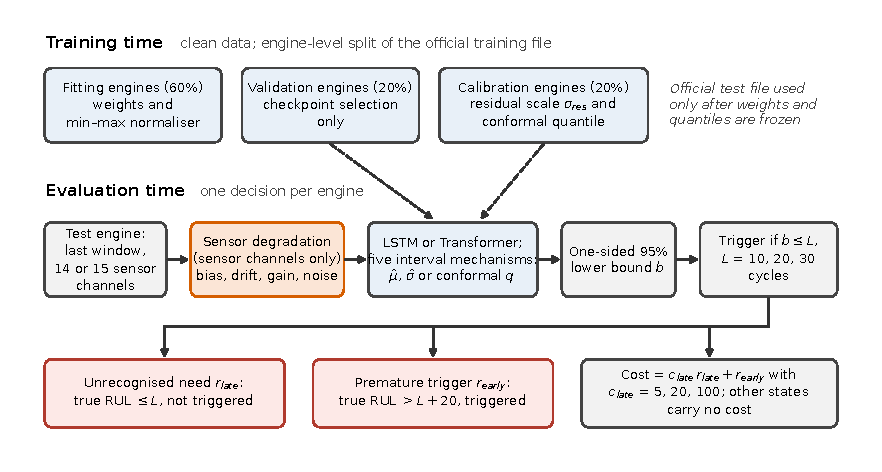
\includegraphics[width=\textwidth]{figures/fig1.pdf}
\caption{Evaluation protocol from clean training-time engine partitions to a single maintenance decision per test engine. The scheme describes the stress test performed here; it is not a deployed monitoring system.}
\label{fig:flow}
\end{figure}

\subsection{Models, calibration and leakage control}
The LSTM has two layers of 64 units with dropout 0.2. The Transformer applies two encoder layers ($d=64$, four heads) with average pooling. Both were trained with Adam for 150 epochs with hyperparameters fixed before the protocol was adopted and not retuned. Five interval mechanisms are built on them: a fixed-variance head (MSE training, one global residual scale), a heteroscedastic Gaussian head (mean and log-scale outputs\cite{nix1994}), MC Dropout ($T=50$, predictive variance including the residual term\cite{gal2016,kendall2017}), a deep ensemble (the five heteroscedastic seeds combined by moment matching\cite{lakshminarayanan2017}) and split conformal prediction with a normalised score (CP-norm\cite{barber2023}).

Figure~\ref{fig:flow} summarises the protocol. Each of five seeds draws its own engine-level partition of the official training file: 60\% of engines fit the weights and the min--max normaliser, 20\% select the checkpoint, and 20\% calibrate the conformal quantile and, for the fixed-variance and MC Dropout mechanisms, the residual scale. The official test file is used once, after all quantities are frozen. Taking the residual scale from the calibration engines rather than from training residuals matters: the calibration-set scale is larger by \NFairRatio\% on average. The protocol repairs an earlier pipeline in which the checkpoint had been selected on the test set. A controlled $2\times2$ retraining with the fitting engines held fixed (Supplement S1) isolates the two choices. On FD001, test-set checkpoint selection lowers RMSE by 1.94 cycles on average over the two normaliser scopes (12.6\% of the validation-selected value) and, with the normaliser scope held fixed, lowers the NASA score by 48.7\% (552.2 to 283.1, fitting-engine normaliser) and 51.9\% (558.4 to 268.4, whole-file normaliser); the normaliser scope moves RMSE by at most \NNormAbsMaxRMSE{} cycles. The intervals analysed here are therefore not products of test-set selection; the models are not state of the art.

\emph{Predicted-mean processing.} The analyses do not clip the predicted mean identically (Supplement S2). The v1.8 clean benchmark clipped every mean to $[0,125]$; the stress-test and decision analyses leave the heteroscedastic mean (also used by CP-norm) and ensemble members unclipped and clip the other means. The clean baseline here is therefore recomputed through the stress-test code path from the released checkpoints (Table~\ref{tab:clean}); the clipped values stay in S2, labelled v1.8 processing. Clipping the heteroscedastic means changes none of the NLL or CP-norm trigger rates in \JClipRateN{} stored cells and the ensemble rates by at most \JClipRateMaxEns{} points, but it changes coverage under a large mean shift by up to \JClipPICPmaxDrift{} (FD002 drift: \JClipDriftTwoU{} unclipped, \JClipDriftTwoA{} clipped). Coverage under shifted inputs therefore depends on this processing; trigger-error direction and size do not.

\subsection{Sensor degradation}
Perturbations act on the raw readings of the sensor channels of the final window before normalisation, without retraining. Operating-setting channels are never perturbed (a diagnostic that perturbs them is summarised in Section~\ref{sec:sens}). Levels are $\{0.1,0.5,1,2,5\}\%$ of each channel's range over the official training file, a fixed fraction of range and not an instrument full scale. \emph{Noise} is additive Gaussian. \emph{Bias} is a constant per-channel offset with a random sign per channel. \emph{Drift} is a linear ramp from zero to the nominal level at the last step of the window, re-zeroed per window, with the same positive sign on every sensor channel. \emph{Gain} multiplies the raw reading by $1\pm k$ with a random sign per channel, so its level is a percentage of the reading, not of the range. Nominal levels of different families are therefore not comparable. Results are related instead through the measured excursion $f_{\mathrm{oob}}$, the fraction of normalised sensor inputs of the terminal windows outside $[-1,1]$, averaged over the same models and realisations as the coverage. Noise, bias and gain use five seeded realisations; drift is deterministic.

Because drift is sign-coherent and bias is not, a drift-versus-bias contrast confounds temporal structure with cross-channel sign coherence. Three controls separate them (Section~\ref{sec:coherent}): a constant $+5\%$ offset on every sensor channel, a constant $-5\%$ offset, and the ramp rerun as a check. Further controls from the earlier analysis (reversed, shuffled, single-channel and continuous-trajectory drift) are summarised in Section~\ref{sec:controls}.

\subsection{Maintenance rule and error accounting}
For each mechanism the rule computes a one-sided 95\% lower bound $b$ on RUL. For the Gaussian mechanisms $b=\hat\mu-1.645\hat\sigma$, which is also the lower limit of their central 90\% interval; coverage (PICP) refers to that central interval. For CP-norm, $b=\hat\mu-q\hat\sigma$ with $q$ the conformal quantile of the \emph{signed} normalised score at level 0.95, recalibrated on the calibration engines, because the central 90\% quantile of the absolute score is not a one-sided 95\% quantile. Maintenance is triggered when $b\le L$, with $L\in\{10,20,30\}$ cycles.

Let $y$ be the true RUL at the evaluated instant. An \emph{unrecognised maintenance need} is $y\le L$ with no trigger; its rate is $r_{\mathrm{late}}$. A \emph{premature trigger} is a trigger with $y>L+20$; its rate is $r_{\mathrm{early}}$. Other states (a trigger with $y\le L$, a trigger with $L<y\le L+20$, no trigger with $y>L$) carry no cost. Both rates use all evaluated engines as denominator; the conditional unrecognised rate uses only engines with $y\le L$. The cost is $c_{\mathrm{late}}r_{\mathrm{late}}+r_{\mathrm{early}}$ with $c_{\mathrm{late}}\in\{5,20,100\}$, a given binary loss and not a maintenance-cost model.

This is a terminal-instant stress test: one decision per engine at one state. It does not simulate the time of first maintenance, availability, safety events or lifetime cost. Where we quote the remaining life of prematurely triggered engines, it is the true remaining life at the evaluated instant (unclipped, official RUL minus one), and the excess over $L$ is what would be forgone if maintenance followed immediately; it is not an estimate of total life lost.

\subsection{Statistical units and uncertainty}
The resampling unit is the engine. Each rate is the mean over engines of the per-engine mean over the five models (and over five realisations for noise and bias). Intervals are percentile intervals from 2000 bootstrap resamples of engines, applied jointly to all mechanisms, conditions and lead times so that comparisons stay paired. They are conditional on the five trained models, whose initialisation and partition variability are confounded; the model-to-model range of each rate is reported separately. Five seeds times the engines is not an independent sample size, and windows are never treated as engines. Rank reversals across cost ratios are counted descriptively; the bootstrap probability that the top mechanism differs is a stability indicator, not a significance test, with no multiplicity correction over the 96 settings. The engine-level analyses of Sections~\ref{sec:coherent}--\ref{sec:cost} were run once on the released checkpoints, are exploratory, and reproduce the released aggregate decision rates (\JAgreeN{} values, maximum absolute difference \JAgreeMax).

\section{Interval reliability under sensor degradation}\label{sec:reliability}
\subsection{Clean baseline}
Table~\ref{tab:clean} summarises clean-input results under fair calibration, recomputed through the same code path and mean processing as the stress tests; the full table is in Supplement S2. Clean coverage lies between \JCleanCovAll{} across mechanisms, backbones and sub-datasets. Relative to the v1.8 benchmark (all means clipped), this lowers PICP in \JCleanAllShiftNchg{} of \JCleanAllShiftN{} cells by at most \JCleanAllShiftMax{} points. Coverage rankings among single-model mechanisms do not transfer between backbones. The deep ensemble has the lowest interval score in all \JEnsBestISeight{} backbone--sub-dataset combinations, but this is an in-sample observation on one ensemble per combination: a paired comparison against independently seeded ensembles favours the ensemble in point estimate on \NIndepPosN{} sub-datasets and excludes zero on \NIndepSigN. The baseline therefore establishes that clean intervals are credible, not which mechanism is best.

\begin{table}[!t]
\caption{Clean-input interval benchmark under fair calibration, recomputed with the stress-test processing of the predicted mean, terminal unit, mean of five seeds. Coverage is the range of PICP over the four sub-datasets; MPIW (cycles) and interval score IS (lower is better) are means over the four sub-datasets. The ensemble is a single $M=5$ estimate.}
\label{tab:clean}
\centering\small
\begin{tabular}{lccc|ccc}
\toprule
 & \multicolumn{3}{c|}{LSTM} & \multicolumn{3}{c}{Transformer} \\
Mechanism & PICP & MPIW & IS & PICP & MPIW & IS \\
\midrule
Fixed variance & 0.87--0.91 & 54 & 76.3 & 0.84--0.92 & 51 & 75.0 \\
Heteroscedastic & 0.86--0.91 & 47 & 68.4 & 0.86--0.89 & 46 & 69.6 \\
MC Dropout & 0.89--0.93 & 56 & 75.5 & 0.88--0.92 & 53 & 69.5 \\
Deep ensemble & 0.91--0.96 & 50 & 63.3 & 0.91--0.93 & 49 & 63.2 \\
Split-CP (norm) & 0.88--0.93 & 51 & 68.2 & 0.86--0.91 & 48 & 69.8 \\
\bottomrule
\end{tabular}
\end{table}

\subsection{Direction and size of coverage failures}
Figure~\ref{fig:foob} plots the coverage of the heteroscedastic head against $f_{\mathrm{oob}}$ for the four families. On six-condition sub-datasets every family loses coverage as $f_{\mathrm{oob}}$ rises, but not at the same rate. At a matched $f_{\mathrm{oob}}$ of 10\% on FD002, coverage (LSTM to Transformer, interpolated between measured levels) is \JMatchDrift{} under drift, \JMatchGain{} under gain, \JMatchNoise{} under additive noise and \JMatchBias{} under bias; on FD004 the matched values are \JMatchFDfourNoise{} (noise), \JMatchFDfourBias{} (bias) and \JMatchFDfourGain{} (gain), and the drift curve ends at 9.2\% so it has no 10\% value. The out-of-range share therefore does not order the damage across families. At equal nominal amplitude (5\% of range) both drift and bias collapse coverage on six-condition data: \JDriftCovTwoSix{} (FD002) and \JDriftCovFourSix{} (FD004) for drift, \JBiasCovSix{} for bias, against clean values of \JCleanCovSix.

\begin{figure}[!t]
\centering
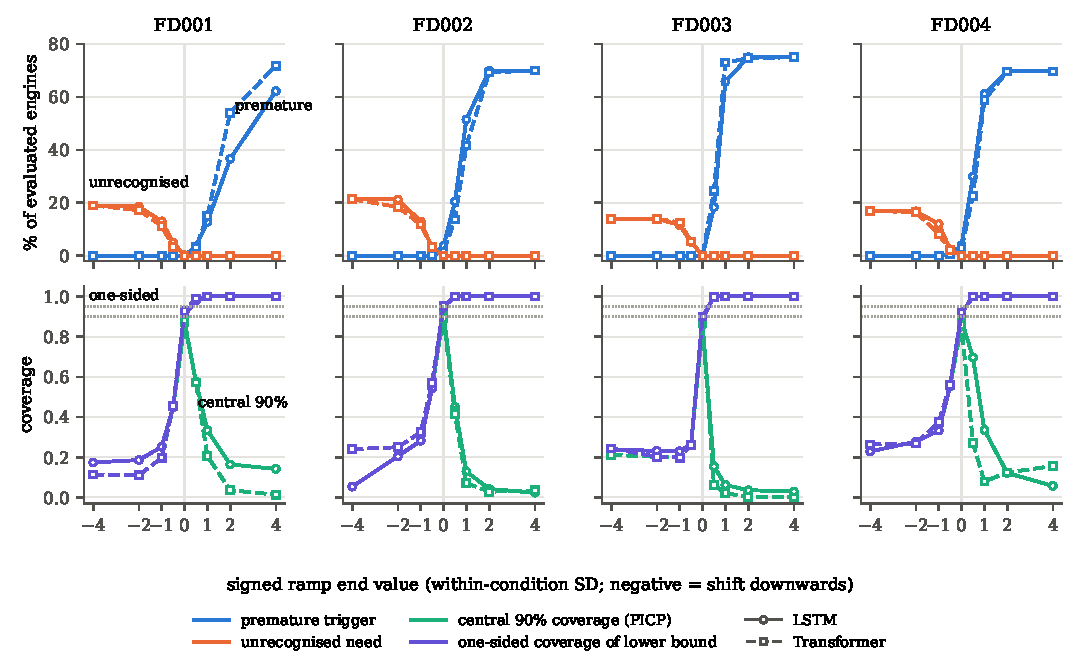
\includegraphics[width=\textwidth]{figures/fig2.pdf}
\caption{Coverage of the 90\% interval (heteroscedastic head) against the fraction of out-of-range normalised sensor inputs, five perturbation levels per curve (0.1 to 5\%; noise, bias and drift as a share of the training range, gain as a share of the reading), mean of five models and, for noise, bias and gain, five realisations. Top: six-condition sub-datasets; bottom: single-condition sub-datasets (zero excursion is drawn at the left edge of the axis). The dotted line marks the 10\% excursion used for comparison in the text.}
\label{fig:foob}
\end{figure}

On single-condition sub-datasets $f_{\mathrm{oob}}$ misses the failure in one direction and flags it in the other. Drift at 5\% lowers coverage from \JCleanCovOne{} to \JDriftCovOne{} on FD001 and from \JCleanCovThree{} to \JDriftCovThree{} on FD003 while $f_{\mathrm{oob}}$ stays below $\JDriftFoobSingleMax$, because windows near end of life already lie inside the training range and a ramp does not push them out. Gain errors, in contrast, move \JGainSingleFoob\% of inputs out of range at the lowest level and collapse coverage (\JGainSinglePICP), so here the excursion does flag the failure. We read $f_{\mathrm{oob}}$ as neither necessary nor sufficient for coverage loss. It relates to coverage within a family but cannot stand in for a family-specific assessment. The earlier crossover summary is replaced by this matched comparison because \JLCcells{} of \JLCtotal{} of its cells were left-censored (Supplement S3).

\subsection{Direction of the shift sets the side of the error}\label{sec:coherent}
The drift ramp is positive on every channel, while bias has a random sign per channel. Table~\ref{tab:coh} shows what a constant offset does. A constant $+5\%$ offset on every sensor channel reproduces the six-condition damage of the ramp: coverage is \JCohPosPICPSix{} against \JCohRampPICPSix{} for the ramp, and premature triggers at $L=20$ are \JCohPosPremSix\% against \JCohRampPremSix\% of evaluated engines (FD002 \JCohPosPremFDtwo\% against \JCohRampPremFDtwo\%; FD004 \JCohPosPremFDfour\% against \JCohRampPremFDfour\%), with no unrecognised need (at most \JCohPosUnrecSixMax\%). On these data the temporal ramp is therefore not needed to reproduce the damage. The mirror-image constant $-5\%$ offset leaves premature triggers at most \JCohNegPremSixMax\% but produces unrecognised needs in \JCohNegUnrecSix\% of evaluated engines (FD002 \JCohNegUnrecFDtwo\%; FD004 \JCohNegUnrecFDfour\%). Random-sign bias of the same magnitude is much less damaging on FD002 (coverage \NBiasEqL{} LSTM, \NBiasEqT{} Transformer, against \JCohPosPICPFDtwo{} for the constant positive offset), so sign coherence, not magnitude alone, sets the damage. On single-condition sub-datasets the ramp is more damaging than the constant offset (coverage \JCohRampPICPOne{} against \JCohPosPICPOne{} on FD001; \JCohRampPICPThree{} against \JCohPosPICPThree{} on FD003). The ramp and the constant offset differ in shape, in mean offset over the window and in distance from the training windows, and these were not separated, so we call this waveform sensitivity and do not attribute it to temporal order. Only three sign patterns (all positive, all negative, random) were tested; which channels carry the effect was not identified.

\begin{table}[!t]
\caption{Sign-coherent shift control, heteroscedastic head, 5\% of range, mean of five models: PICP / premature (\%) / unrecognised (\%) at $L=20$. Ramp: the drift family; constant: the same offset on every sensor channel and step. Exploratory, inference only.}
\label{tab:coh}
\centering\footnotesize
\begin{tabular}{lcccc}
\toprule
 & Clean PICP & Ramp (+) & Constant $+5\%$ & Constant $-5\%$ \\
\midrule
LSTM FD001 & 0.86 & 0.64 / 3 / 0.0 & 0.75 / 2 / 0.0 & 0.65 / 0 / 3.0 \\
LSTM FD002 & 0.91 & 0.05 / 69 / 0.0 & 0.04 / 63 / 0.0 & 0.31 / 2 / 12.2 \\
LSTM FD003 & 0.86 & 0.21 / 14 / 0.0 & 0.82 / 0 / 0.0 & 0.67 / 0 / 0.4 \\
LSTM FD004 & 0.88 & 0.31 / 59 / 0.0 & 0.35 / 33 / 0.0 & 0.66 / 3 / 3.7 \\
\midrule
Transformer FD001 & 0.88 & 0.64 / 2 / 0.0 & 0.85 / 0 / 0.0 & 0.74 / 0 / 1.0 \\
Transformer FD002 & 0.89 & 0.03 / 69 / 0.0 & 0.02 / 66 / 0.0 & 0.28 / 0 / 14.8 \\
Transformer FD003 & 0.87 & 0.10 / 17 / 0.0 & 0.69 / 1 / 0.0 & 0.74 / 0 / 0.4 \\
Transformer FD004 & 0.86 & 0.05 / 52 / 0.0 & 0.10 / 36 / 0.0 & 0.57 / 3 / 7.8 \\
\bottomrule
\end{tabular}
\end{table}

\subsection{Waveform controls}\label{sec:controls}
Controls from the earlier analysis vary the waveform of the 5\% shift on FD001 and FD002 for both backbones (released result files; Supplement S5). On FD001 a shuffled ramp (same values, random order) leaves coverage at \JWFoneShuf{} against \JWFoneClean{} clean, whereas the ramp gives \JWFoneRamp{}, the reversed ramp \JWFoneRev{} and a per-trajectory ramp \JWFoneCont. On FD002 shuffling spares neither backbone: coverage is \JWFtwoShufL{} (LSTM) and \JWFtwoShufT{} (Transformer) against \NRampL{} and \NRampT{} for the ramp; a reversed ramp leaves \NRevL{} and \NRevT, and fixing the last $k$ steps of the shuffled ramp gives \NFixEndOneL{} ($k=1$) and \NFixEndFiveL{} ($k=5$) for the LSTM and \NFixEndT{} for the Transformer. The evidence thus supports damage that depends on waveform and end-of-window offset, differently by dataset and backbone: shuffling spares both backbones on FD001, the LSTM only partly on FD002 and the Transformer not at all. These controls change end value, energy and order together; they do not identify temporal order as the mechanism or show that the models read a trend as degradation.

\subsection{Additive noise: mean and scale contributions}\label{sec:noise}
Supporting result, bounded claim. A four-way frozen-output decomposition under additive noise (mean and scale outputs each taken from the clean or perturbed condition, where the heteroscedastic head has lost ten points of coverage) attributes the loss predominantly to the mean output. In all 16 backbone--sub-dataset--mechanism cells the pooled point estimate of the mean effect exceeds the scale effect in magnitude under both decomposition orders, and a per-seed paired bootstrap excludes zero in \NCITot{} of 32 order-specific cells. The sign of the scale effect depends on the order: read with the mean varied first the learned scale helps in \NHelpA{} cells, read with the scale varied first it is harmful in all 16. There is no order-independent evidence that the learned scale helps, and the interaction between mean and scale is positive in all 16 cells. This concerns additive noise at one operating point; Section~\ref{sec:swap} performs its own swap for bias and drift.

\section{Maintenance-trigger errors and cost sensitivity}\label{sec:decision}
\subsection{Both errors, with engine-level uncertainty}
Table~\ref{tab:dec} and Figure~\ref{fig:dec}a,b give the heteroscedastic head at $L=20$. Under the sign-coherent positive drift on six-condition sub-datasets, premature triggers reach \JDriftPremRange\% of evaluated engines. Engine-level 95\% intervals span \JDriftPremCI\% over the four cells (half-width at most \JDriftPremHalfCI{} points), and the model-to-model range is \JDriftPremModelRange\%. No unrecognised need occurs: the rate is at most \JDriftUnrecMax\% in every one of the five mechanisms, eight backbone--sub-dataset pairs and three lead times. Premature rates under drift range \JDriftPremAllMech\% across the five mechanisms, so the choice of mechanism does not remove the error. The prematurely triggered engines have a mean unclipped true remaining life of \JDriftRULunc{} cycles (\JDriftRULcap{} clipped), far from needing maintenance. On single-condition sub-datasets drift triggers prematurely on \JDriftPremSingle\% (FD001, LSTM and Transformer) and \JDriftPremSingleThree\% (FD003) of engines.

\begin{table}[!t]
\caption{Terminal-instant decision stress test, heteroscedastic head, six-condition sub-datasets, $L=20$, one-sided 95\% lower bound. Rates are percentages of evaluated engines with engine-bootstrap 95\% intervals in brackets (2000 resamples, conditional on the five trained models); ``models'' is the range of the premature rate over the five models; ``cond.'' is the unrecognised rate among engines with true RUL $\le L$. Remaining life is the mean unclipped true RUL at the evaluated instant among prematurely triggered engines. All mechanisms and lead times: Supplement S4.}
\label{tab:dec}
\centering\footnotesize
\begin{tabular}{llcccccc}
\toprule
Cell & Condition & Premature (\%) & Models & Unrecognised (\%) & Cond.\ (\%) & Remaining life \\
\midrule
LSTM FD002 & Clean & 4 [2, 6] & 1--6 & 0.0 [0.0, 0.0] & 0 & 49 [46, 53] \\
LSTM FD002 & Drift 5\% & 69 [64, 75] & 69--70 & 0.0 [0.0, 0.0] & 0 & 105 [99, 111] \\
LSTM FD002 & Bias 5\% & 17 [15, 18] & 14--28 & 7.8 [5.8, 10.0] & 37 & 104 [98, 110] \\
\midrule
LSTM FD004 & Clean & 4 [2, 6] & 2--5 & 0.1 [0.0, 0.3] & 0 & 60 [51, 71] \\
LSTM FD004 & Drift 5\% & 59 [53, 64] & 51--65 & 0.0 [0.0, 0.0] & 0 & 105 [99, 111] \\
LSTM FD004 & Bias 5\% & 30 [27, 33] & 25--33 & 2.5 [1.7, 3.5] & 15 & 103 [97, 109] \\
\midrule
Transformer FD002 & Clean & 2 [0, 3] & 1--2 & 0.1 [0.0, 0.2] & 0 & 47 [44, 52] \\
Transformer FD002 & Drift 5\% & 69 [64, 74] & 68--70 & 0.0 [0.0, 0.0] & 0 & 105 [99, 111] \\
Transformer FD002 & Bias 5\% & 14 [13, 15] & 13--15 & 10.2 [7.7, 13.1] & 48 & 104 [98, 110] \\
\midrule
Transformer FD004 & Clean & 3 [1, 5] & 2--5 & 0.0 [0.0, 0.0] & 0 & 64 [54, 76] \\
Transformer FD004 & Drift 5\% & 52 [47, 58] & 47--59 & 0.0 [0.0, 0.0] & 0 & 101 [95, 107] \\
Transformer FD004 & Bias 5\% & 32 [29, 35] & 27--34 & 1.8 [1.2, 2.4] & 11 & 105 [99, 111] \\
\bottomrule
\end{tabular}
\end{table}

Random-sign bias errs on both sides, at lower rates than the positive drift. Premature triggers are \JBiasPremRange\% (all mechanisms \JBiasPremAllMech\%) and unrecognised needs \JBiasUnrecRange\% of evaluated engines, equivalent to \JBiasUnrecCondRange\% of the engines with true RUL $\le L$ (all mechanisms \JBiasUnrecAllMech\%). For the heteroscedastic head on the six-condition cells, clean inputs give \JCleanPremRange\% premature triggers and at most \JCleanUnrecMax\% unrecognised needs; noise at 1\% of range gives \JNoisePremRange\% premature triggers. The side of the error therefore depends on the sign pattern of the shift (Section~\ref{sec:coherent}): a decision audit has to count both sides, and a coverage figure does not say which side fails. The premature rates under drift vary with the lead time (\JDriftPremLten\% at $L=10$, \JDriftPremLthirty\% at $L=30$ over the four six-condition cells; Figure~\ref{fig:dec}c).

\begin{figure}[!t]
\centering
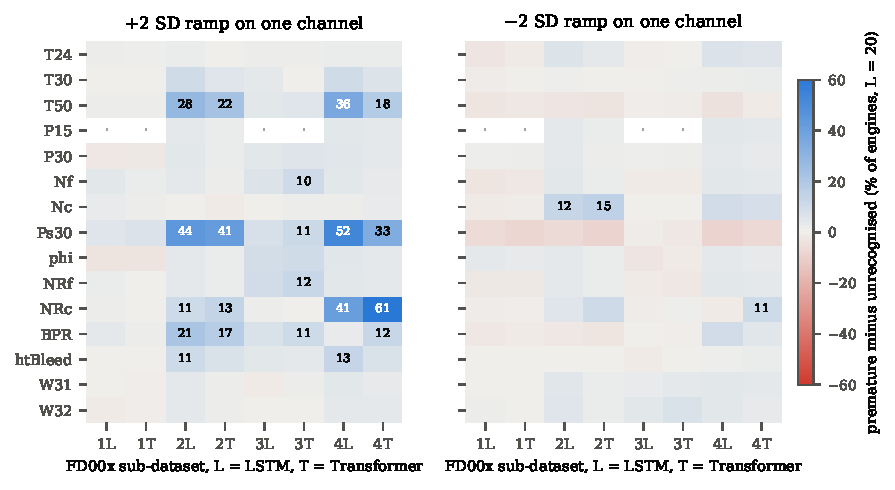
\includegraphics[width=\textwidth]{figures/fig3.pdf}
\caption{(a, b) Premature triggers and unrecognised needs of the heteroscedastic head at $L=20$ for each sub-dataset and condition; circles: LSTM, squares: Transformer; bars are engine-bootstrap 95\% intervals. (c) Lead-time dependence on the four six-condition cells; thin lines are individual cells, thick lines their mean. (d) Number of the 24 backbone--sub-dataset--lead-time cases per condition in which the ranking of the five mechanisms (solid) or only its top place (hatched) differs between cost ratios 5, 20 and 100.}
\label{fig:dec}
\end{figure}

\subsection{Mean or scale: an output swap at the decision point}\label{sec:swap}
A contracted scale raises the lower bound, so scale contraction alone cannot trigger earlier; an expanded scale can. Mean and scale of the heteroscedastic head were each taken from the clean or the perturbed condition of the same model. On six-condition sub-datasets the mean under positive drift falls by $\JMuShiftDrift$ cycles on average; changing only the mean raises premature triggers by \JSwapMuDrift{} points (lower interval limits at least \JSwapMuDriftLoCI{}), whereas changing the scale given the perturbed mean moves them by $\JSwapSigDrift$ points, at most \JSigExtMaxPt{} (\JSigExtMaxCell; interval \JSigExtMaxLo{} to \JSigExtMaxHi). On single-condition sub-datasets the scale contracts and offsets part of the mean effect in \JSwapSigDriftSingleN{} of four cases ($\JSwapSigDriftSingle$ points against a mean effect of \JSwapMuDriftSingle{}; largest \JSigExtMinPt{} for \JSigExtMinCell, interval \JSigExtMinLo{} to \JSigExtMinHi), which keeps premature rates low there. The scale-effect interval excludes zero in \JSigExtExclZero{} of \JSigExtCells{} cells, so the scale is not negligible. For random-sign bias the mean adds \JSwapMuBias{} points of premature triggers and \JSwapMuBiasUnrec{} points of unrecognised needs; the scale alone moves the unrecognised rate by $\JSwapSigBiasUnrec$ points. For the constant offsets of Section~\ref{sec:coherent} (Supplement S5), on six-condition data the mean effect is \JCPswapMuPrem{} points of premature triggers for $+5\%$ (scale effect \JCPswapSigPrem) and \JCNswapMuUnrec{} points of unrecognised needs for $-5\%$ (scale effect \JCNswapSigUnrec). The swaps identify the mean shift as the main driver, with scale changes of \JSigExtMinPt{} to \JSigExtMaxPt{} points at the extremes. This is an output-level decomposition, not a physical mechanism.

\subsection{Cost ratios and mechanism rankings}\label{sec:cost}
Across \JRevGroups{} backbone--sub-dataset--condition--lead-time groups, the cost ranking of the five mechanisms changes between cost ratios 5, 20 and 100 in \JRevTotal{} and the top-ranked mechanism changes in \JTopTotal. By condition (Figure~\ref{fig:dec}d), the full ranking changes in \JRevBias{} of \JNBias{} bias cases, \JRevNoise{} noise, \JRevClean{} clean and \JRevDrift{} drift cases; the top place changes in \JTopBias, \JTopNoise, \JTopClean{} and \JTopDrift{} cases respectively. Under drift the unrecognised rate is zero, so the cost is the same at every ratio and the ranking is the ranking of premature rates. Where the top place changes, the engine-bootstrap probability that the top mechanism at ratio 5 differs from that at ratio 100 has median \JTopBootMed{} (interquartile range \JTopBootIQR; at least 0.5 in \JTopBootGeFive of \JTopBootN{} cases). This describes how often resampling engines preserves the observed change of top place, conditional on the five models; it is not a significance test, and the probabilities for all 96 settings are in the supplementary CSV. The released per-engine bootstrap of the top mechanism against the other four excludes zero in only \NBootSig{} of 144 comparisons per backbone--sub-dataset. No mechanism is recommended on cost alone.

\subsection{Sensitivity checks}\label{sec:sens}
Perturbing the three operating-setting channels in addition to the sensors raised the premature rate under drift on FD004 from \NAOneFDfourSens{} (sensors only) to \NAOneFDfourJoint, while perturbing the settings alone gave \NAOneFDfourSet{}; on FD002 the two are indistinguishable (\NAOneFDtwoSens{} against \NAOneFDtwoJoint). The sensor-only premature rate is therefore the lower of the two in this FD004 check; this tested sensitivity does not make the sensor-only figures conservative in general. Engines with fewer than 30 cycles are excluded (\JExclTwo{} of 259 for FD002, \JExclFour{} of 248 for FD004); the effect of including them with padding was not assessed. Label-instant sensitivity is at most \JLabelHeadline{} points (Section~\ref{sec:framework}).

\section{Discussion and limitations}
\subsection{What the results change in evaluation practice}
Four practices follow from the evidence, within the conditions tested. First, an interval that feeds a maintenance rule should be evaluated through the rule: both trigger errors, premature and unrecognised, should be reported beside coverage, with engine-level intervals. Coverage was lost under drift and under bias, yet the lower bound erred on the premature side for one sign of shift and on the late side for the other. Second, the share of out-of-range inputs should not be read as a risk indicator; it missed drift on single-condition data and ordered the perturbation families inconsistently on six-condition data. Third, robustness tests should vary the sign pattern of a shift across channels, because the direction of the trigger error followed it; testing only random-sign offsets would have shown coverage of \NBiasEqT--\NBiasEqL{} on FD002 where a coherent positive shift of equal magnitude gave \JCohPosPICPFDtwo. Fourth, mechanisms should not be selected on a single cost ratio: rankings changed with the ratio in \JRevTotal{} of \JRevGroups{} settings, and under drift they did not change only because no mechanism produced a late error.

\subsection{What cannot be inferred}
The results do not show that real sensor drift resembles a positive ramp on every channel; sensor physics is not modelled. They do not show that deployed systems fail in these ways or give a safety margin: one terminal decision per engine says nothing about first-maintenance time, availability or lifetime cost, and the cost is a binary loss. The output swap does not identify a physical mechanism, nor does it show that the models read a shift as degradation; a monitor separating sensor drift from genuine degradation, which also trends, is a separate problem. The results do not extend to N-CMAPSS, other backbones, other rules or other lead-time families.

\subsection{Limitations}
The data are simulated, and two backbones with fixed hyperparameters were studied. The five models of each backbone use five partitions, so the engine-level intervals are conditional on those models, and initialisation and partition variability are confounded. Perturbation levels are fractions of the training range, not calibrated to any instrument; noise, bias and gain have five realisations each, and the sign patterns of Section~\ref{sec:coherent} are limited to three. Engines with fewer than 30 cycles were excluded. The predicted mean is clipped in some mechanisms and not in others (Section~\ref{sec:framework}); coverage under large mean shifts depends on this, and trigger rates of the heteroscedastic head and CP-norm do not. The waveform controls (FD001 and FD002 only; fixed-end shuffle FD002 only) change end value, energy and order together, so temporal order is not identified as a cause. The engine-level analyses were run once, are exploratory and not pre-registered; rank-reversal counts are descriptive. The literature comparison rests on a bounded search. Reproducibility is layered: released result files regenerate the v1.8 tables; the engine-level analyses rerun inference from released checkpoints and reproduce the released aggregate rates; training and a few intermediate files are not covered.

\section{Conclusion}
In this C-MAPSS stress test, three bounded conclusions hold. First, coverage and the share of out-of-range inputs do not tell which way an interval-based maintenance rule fails: at matched excursion, drift and bias differed widely in coverage, and a sign-coherent positive shift gave premature triggers in \JDriftPremRange\% of evaluated six-condition engines at a 20-cycle lead time with no unrecognised need, while the opposite sign gave unrecognised needs. Second, output swaps identified the mean shift as the main driver of these errors, with scale changes shifting premature rates by between \JSigExtMinPt{} and \JSigExtMaxPt{} points under drift; under additive noise the scale effect has no order-independent sign. Third, no interval mechanism is recommendable on cost alone, since cost rankings changed across cost ratios in \JRevTotal{} of \JRevGroups{} settings and not at all under drift. Evaluations of intervals used for maintenance should therefore report both trigger errors with engine-level uncertainty; whether the same holds on recorded flight data or other rules remains open.

\section*{Statements and Declarations}
\noindent\textbf{Ethical considerations.} Not applicable; the study uses a public simulated dataset and involves no human or animal subjects.\\[2pt]
\noindent\textbf{Consent to participate.} Not applicable.\\[2pt]
\noindent\textbf{Consent for publication.} Not applicable.\\[2pt]
\noindent\textbf{Declaration of conflicting interest.} The author declared no potential conflicts of interest with respect to the research, authorship and/or publication of this article.\\[2pt]
\noindent\textbf{Funding statement.} The author received no financial support for the research, authorship and/or publication of this article.\\[2pt]
\noindent\textbf{Declaration of generative AI use.} The AI assistant Claude (Anthropic) was used to help write and run the analysis code, to restructure and edit the text, and to check numbers and cross-references against result files. The author designed the study, reviewed and verified all outputs, and takes full responsibility for the content of the article. No AI tool is listed as an author.\\[2pt]
\noindent\textbf{Data availability.} The C-MAPSS data are available from the NASA Prognostics Center of Excellence. Code, trained checkpoints, result files and the scripts that generate the tables and numbers of this paper are in the public repository \ifanon given to the editor\else\url{https://github.com/jeff-1980/paper2-JRR}\fi. Its result files regenerate the original tables; the per-engine analyses rerun inference from the released checkpoints. Model training, latency and cross-platform reproduction are not covered, and a few intermediate files read by the original pipeline are not released.


\begin{thebibliography}{99}
\small
\setlength{\itemsep}{0pt}
\bibitem{peng2019} Peng W, Ye ZS, Chen N. Bayesian deep-learning-based health prognostics toward prognostics uncertainty. IEEE Trans Ind Electron 2020; 67: 2283–2293. DOI: 10.1109/TIE.2019.2907440.
\bibitem{basora2025} Basora L, Viens A, Chao MA, Olive X. A benchmark on uncertainty quantification for deep learning prognostics. Reliab Eng Syst Saf 2025; 253: 110513. DOI: 10.1016/j.ress.2024.110513.
\bibitem{zhan2024} Zhan Y, Kong Z, Wang Z, Jin X, Xu Z. Remaining useful life prediction with uncertainty quantification based on multi-distribution fusion structure. Reliab Eng Syst Saf 2024; 251: 110383. DOI: 10.1016/j.ress.2024.110383.
\bibitem{piao2025} Piao S, Huang R, Tsung F. CRULP: Reliable RUL Estimation Inspired by Conformal Prediction. IEEE Trans. Instrum. Meas. 2025; 74: 1–11. DOI: 10.1109/tim.2024.3522678.
\bibitem{mao2024} Mao S, Li X, Zhao B. Remaining useful life prediction based on time-series features and conformalized quantile regression. Meas. Sci. Technol. 2024; 35: 126113. DOI: 10.1088/1361-6501/ad762c.
\bibitem{xu2021} Xu Z, Guo Y, Saleh JH. Accurate Remaining Useful Life Prediction With Uncertainty Quantification: A Deep Learning and Nonstationary Gaussian Process Approach. IEEE Trans Reliab 2022; 71(1): 443–456. DOI: 10.1109/tr.2021.3124944.
\bibitem{xu2026} Xu W, Gao S, Wang Z, Zio E. A novel uncertainty-aware framework for remaining useful life prediction integrating uncertainty quantification and calibration. Reliab Eng Syst Saf 2026; 275: 112763. DOI: 10.1016/j.ress.2026.112763.
\bibitem{xu2023} Li X, Xu Y, Li N, Yang B, Lei Y. Remaining Useful Life Prediction With Partial Sensor Malfunctions Using Deep Adversarial Networks. IEEE/CAA J Autom Sinica 2023; 10(1): 121–134. DOI: 10.1109/jas.2022.105935.
\bibitem{tang2026} Tang D. A deep learning framework for remaining useful life prediction of turbofan engines with partial sensor failure. PLoS One 2026; 21(4): e0347312. DOI: 10.1371/journal.pone.0347312.
\bibitem{hachem2024} Hachem H, Vu HC, Fouladirad M. Different methods for RUL prediction considering sensor degradation. Reliab. Eng. Syst. Saf. 2024; 243: 109897. DOI: 10.1016/j.ress.2023.109897.
\bibitem{kim2020} Kim M, Liu K. A Bayesian deep learning framework for interval estimation of remaining useful life in complex systems by incorporating general degradation characteristics. IISE Trans 2020; 53(3): 326–340. DOI: 10.1080/24725854.2020.1766729.
\bibitem{lee2022} Lee J, Mitici M. Deep reinforcement learning for predictive aircraft maintenance using probabilistic Remaining-Useful-Life prognostics. Reliab Eng Syst Saf 2023; 230: 108908. DOI: 10.1016/j.ress.2022.108908.
\bibitem{zhu2025} Zhu Z, Wang L, Chen M, Zhao X. Predictive Maintenance Strategies for Aero‐Engines Considering Remaining Useful Life Prediction Interval. Qual Reliab Eng Int 2025; 41(8): 3350–3359. DOI: 10.1002/qre.70043.
\bibitem{saxena2008} Saxena A, Goebel K, Simon D, Eklund N. Damage propagation modeling for aircraft engine run-to-failure simulation. Proc 1st Int Conf Prognostics Health Manag (PHM) 2008: 1–9.
\bibitem{nix1994} Nix DA, Weigend AS. Estimating the mean and variance of the target probability distribution. Proc IEEE Int Conf Neural Networks (ICNN) 1994: 55–60. DOI: 10.1109/ICNN.1994.374138.
\bibitem{gal2016} Gal Y, Ghahramani Z. Dropout as a Bayesian approximation: representing model uncertainty in deep learning. Proc Int Conf Mach Learn (ICML) 2016; 48: 1050–1059.
\bibitem{kendall2017} Kendall A, Gal Y. What uncertainties do we need in Bayesian deep learning for computer vision?. Adv Neural Inf Process Syst 2017; 30.
\bibitem{lakshminarayanan2017} Lakshminarayanan B, Pritzel A, Blundell C. Simple and scalable predictive uncertainty estimation using deep ensembles. Adv Neural Inf Process Syst 2017; 30.
\bibitem{barber2023} Barber RF, Candès EJ, Ramdas A, Tibshirani RJ. Conformal prediction beyond exchangeability. Ann Stat 2023; 51: 816–845.
\end{thebibliography}

\end{document}

